\documentclass{beamer}
\usepackage{xeCJK}
\hypersetup{colorlinks,linkcolor=}

\usetheme{CambridgeUS}
\title{Bit-true arithmetics}
\author[jdh8]{何震邦 (Chen-Pang He, jdh8)}
\date{March 19, 2025}
\institute{Skymizer}

\begin{document}
\maketitle

\begin{frame}{Quantization}
    \begin{itemize}
        \item Quantization maps a large/continuous set to a small/countable set.
        \item Quantization is required because we only have finite bits to store data.
        \item Further quantization reduces space and probably time usage.
    \end{itemize}
\end{frame}

\begin{frame}{Accuracy and precision}
    \begin{figure}
        \caption{
            \href
                {https://en.wikipedia.org/wiki/Accuracy_and_precision\#ISO_definition_(ISO_5725)}
                {Accuracy according to BIPM and ISO 5725}
        }
        \begin{minipage}{0.4\textwidth}
            \centering
            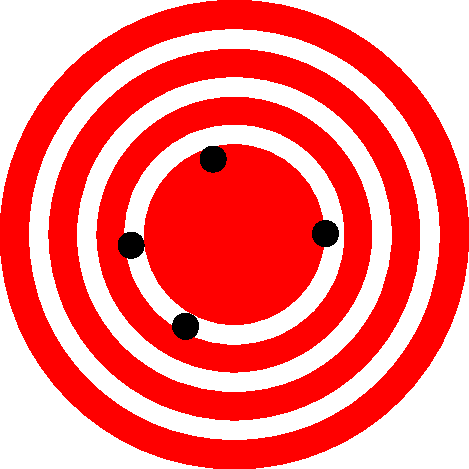
\includegraphics[width=0.8\textwidth]{assets/High_accuracy_Low_precision.pdf} \\
            Low accuracy due to low precision
        \end{minipage}
        \begin{minipage}{0.4\textwidth}
            \centering
            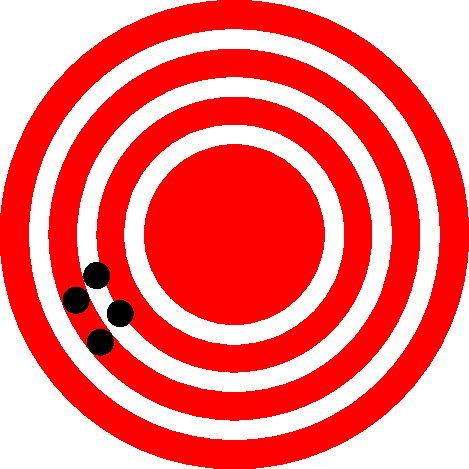
\includegraphics[width=0.8\textwidth]{assets/High_precision_Low_accuracy.pdf} \\
            Low accuracy despite of high precision
        \end{minipage}
    \end{figure}
\end{frame}

\begin{frame}{Rounding mode}
    \begin{figure}
        \href
            {https://upload.wikimedia.org/wikipedia/commons/8/8a/Comparison_rounding_graphs_SMIL.svg}
            {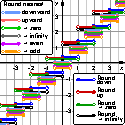
\includegraphics[height=0.625\textheight]{assets/Comparison_rounding_graphs_SMIL.pdf}}

        \caption{
            \href{https://upload.wikimedia.org/wikipedia/commons/8/8a/Comparison_rounding_graphs_SMIL.svg}{Interactive graph}
            by CMG Lee on
            \href{https://commons.wikimedia.org/wiki/File:Comparison_rounding_graphs_SMIL.svg}{Wikimedia Commons}
        }
    \end{figure}
\end{frame}

\end{document}